\documentclass[aspectratio=169]{beamer}

\usepackage[utf8]{inputenc}
\usepackage[T1]{fontenc}
\usepackage[french]{babel}

\usepackage{./pkg/commonstyles}
\usepackage{./pkg/presstyle}

\usepackage{vdr}	

\usepackage{pgfplots}
\usepgfplotslibrary{groupplots}
\usetikzlibrary{backgrounds}
\usetikzlibrary{positioning}
\usepackage[list-style=itemize, backref=true, mark-format={ }]{enotez}

\usetikzlibrary{external}
\tikzsetexternalprefix{pdffig/}
%\tikzexternalize

\title{VDR-4 -- Imagier}
\institute{}
\titlegraphic{}

\begin{document}

\maketitle

\begin{frame}{Cycle à haute et basse fréquence}
	\pgfplotsset{
	lfhf/.style={
		height = 0.42 \textheight,
		enlarge y limits = {value=0.9, upper},
		},
}
\tikzset{
	zoomline/.style={
		opacity=1,
		dotted
	},
	}

\def\zstart{7.2}
\def\zend{7.8}
\newcommand{\istart}{2}
\newcommand{\tic}{2}
\newcommand{\pstart}{7.365}
\newcommand{\tip}{0.059}

\begin{tikzpicture}
	\begin{groupplot}[
			group style={
				group size=1 by 2,
				y descriptions at=edge left,
				xlabels at=edge bottom
				},
				ylabel=Pression (hPa),
				xlabel=Temps (s),
				max space between ticks=40
			]
		\nextgroupplot[lfhf]

		\addplot []table[x=time, y=Pao] {dat/simvent1.dat};


		\coordinate (PSO) at (axis cs:\zstart,0);
		\coordinate (PSE) at (axis cs:\zend,0);
		\coordinate (PNO) at (axis cs:\zstart,\pgfkeysvalueof{/pgfplots/ymax});
		\coordinate (PNE) at (axis cs:\zend,\pgfkeysvalueof{/pgfplots/ymax});

		\draw [plage](axis cs:\istart,45) -- (axis cs:\istart + \tic, 45) node[midway, above] {Inspi.};
		\draw [plage](axis cs:\istart + \tic,45) -- (axis cs:\istart + 2*\tic, 45) node[midway, above] {Expi.};

		\draw [dashed] 
		(axis cs: \istart,\pgfkeysvalueof{/pgfplots/ymax}) -- (axis cs:\istart,0)
	 	(axis cs: \istart + \tic,\pgfkeysvalueof{/pgfplots/ymax}) -- (axis cs:\istart + \tic,0)
		(axis cs: \istart + 2 *\tic,\pgfkeysvalueof{/pgfplots/ymax}) -- (axis cs:\istart + 2*\tic,0);

		%\fill [opacity=0.15] (PSO) rectangle (PNE);
		\draw [zoomline] (PSO) rectangle (PNE);


		\nextgroupplot[lfhf,
				max space between ticks=80,
				width=0.75\textwidth,
				axis background/.style={fill=gray!15, opacity=0.8},
				]
		\addplot [restrict x to domain=\zstart:\zend]table[x=time, y=Pao] {dat/simvent1.dat};

		\coordinate (ZNO) at (axis cs:\zstart,\pgfkeysvalueof{/pgfplots/ymax});
		\coordinate (ZNE) at (axis cs:\zend,\pgfkeysvalueof{/pgfplots/ymax});
		\coordinate (ZSO) at (axis cs:\zstart,\pgfkeysvalueof{/pgfplots/ymin});
		\coordinate (ZSE) at (axis cs:\zend,\pgfkeysvalueof{/pgfplots/ymin});


		\draw [dashed] 
		(axis cs: \pstart,\pgfkeysvalueof{/pgfplots/ymax}) -- (axis cs:\pstart,0)
		(axis cs: \pstart + \tip,\pgfkeysvalueof{/pgfplots/ymax}) -- (axis cs:\pstart + \tip,0)
		(axis cs: \pstart + 2 *\tip,\pgfkeysvalueof{/pgfplots/ymax}) -- (axis cs:\pstart + 2*\tip,0);
		\draw [plage] (axis cs:\pstart,45) -- (axis cs:\pstart + \tip, 45) node[midway, above] {Ins.};
		\draw [plage](axis cs:\pstart + \tip,45) -- (axis cs:\pstart + 2*\tip, 45) node[midway, above] {Exp.};

	\end{groupplot}

	\begin{scope}[on background layer]
		%\fill [opacity=0.03](ZNO) -- (PNO) -- (PNE) -- (ZNE) -- (ZNO);
		%\fill [opacity=0.03](ZSO) -- (PSO) -- (PNO) -- (PNE) -- (PSE) -- (ZSE) -- (ZSO);
		\fill [opacity=0.1](PSO) -- (PNO) -- (PNE) -- (PSE);
		%\fill [opacity=0.05](ZNE) -- (PNE) -- (PSE) -- (ZSE) -- (ZNE);
		\draw [zoomline](ZNO) -- (PNO) (PNE) -- (ZNE) ;
		\draw [zoomline](ZSO) -- (PSO) (PSE) -- (ZSE) ;
	\end{scope}

\end{tikzpicture}

\end{frame}

\begin{frame}{Fonctionnement du phasitron}
	\begin{columns}
	\column{0.5\textwidth}
	\begin{block}{Insuflation}
		\vspace{.25cm}
	\begin{tikzpicture}[
			scale=.60,
			every node/.style={transform shape}
			]

	\pic [name=P, draw=black!50, fill=gray!10] {phasitron-coupe};
	\pic {venturi-avance};
	\path (P-S) -- (P-Pt) 
		node [pos=0.32] (J) {}
		coordinate [pos=0.15] (D)
		;


		\draw [structure, line width=.2mm, ->] (P-S) ++(3mm,0) to (D);
		\draw [
			structure, 
			line width=.2mm,
			->, 
shorten <=1mm,
			] (D) to (J);

		\draw [
			structure, 
			line width=.5mm, 
			->, 
			out=90, 
			in=-45,
			shorten >=1mm
		] (P-A) ++ (0, -3mm)  to (J);

		\draw [structure, line width=1mm, ->] (J)  to (P-Pt);
	
\end{tikzpicture}
	\end{block}

%%%%%%%%%%%%%%%%%%%%%%%%%%%%%%%%%%%%%%%%%%%%%%%%%%%%%%%%%5
%%%%%%%%%%%%%%%%%%%%%%%%%%%%%%%%%%%%%%%%%%%%%%%%%%%%%%%%%5

	\column{0.5\textwidth}
	\begin{block}{Expiration}
		\vspace{.25cm}

	\begin{tikzpicture}[
			scale=.60,
			every node/.style={transform shape}
			]

	\pic [name=P, draw=black!50, fill=gray!10] {phasitron-coupe};
	\pic {venturi-recule};

		\draw [
			structure,
			line width=1mm, 
			->, 
			out=0, 
			in=90, 
			looseness=1.8,
			] ([yshift=-4mm]P-Pt) to (P-E);

\end{tikzpicture}
	\end{block}
\end{columns}

\end{frame}

\begin{frame}{Pressions moyennes}
	\newcommand{\pexp}{5}
\newcommand{\pins}{18}
\newcommand{\arrpos}{1.06}
\begin{tikzpicture}[
		pline/.style={
			help lines,
			turquoisechum,
			rounded corners,
			out=0,
			in=180,
			thick
			},
		p/.style={
			circle,
			draw=turquoisechum,
			inner sep=0.5mm,
			thick
			}
	]

	\begin{axis}[
		width=0.65\textwidth,
		name=plot,
		font=\scriptsize,
		try min ticks=6,
		xtick={0,4,8},
		ytick={0,30},
		axis x line=bottom,
		axis y line=middle,
		enlarge y limits={value=0.25, upper},
		enlarge x limits={value=0.05, upper},
		extra y ticks={5, 18},
		extra y tick labels={$P_{ins. moy.}$, $P_{exp. moy.}$},
		extra y tick style={grid=major},
		major grid style={turquoisechum, thick}
		]

		\addplot [
			bleufoncechum,
			restrict x to domain=0:8,
			] table[x=time, y=Pao] {dat/f300.dat};

		\coordinate (D) at (axis cs: \pgfkeysvalueof{/pgfplots/xmax},\pins);
		\coordinate (B) at (axis cs: \pgfkeysvalueof{/pgfplots/xmax},\pexp);

	\end{axis}

	\pic [opacity=0.99, name=mm] at ([xshift=3.2cm, yshift=-.95cm]plot.east) {multimeter};

		\node [grad] (mmg50) at (mmscreen.north west) {50};
		\node [grad] (mmg0) at (mmscreen.south west) {0};
		\draw [pScale]	(mmg0) -- (mmg50) node [grad, left=0.0mm, pos=0.6, inner sep=0mm] {30};

		\node [below, white, align=left, font=\tiny] at (mmscreen.south) {Percussionaire\\Corporation};

	\node [p] (pmi) at (mmPmi) {\pins};
	\node [p] (pme) at (mmPme) {\pexp};

	%\draw [pline] (D) -- ([xshift=4mm]D) |- (pmi);
	%\draw [pline] (B) -- ([xshift=5mm]B) |- (pme);

	\draw [pline] (D) to (pmi);
	\draw [pline] (B) to (pme);
\end{tikzpicture}

\end{frame}

\begin{frame}{Pression motrice}
	\newcommand{\pexp}{5}
\newcommand{\pins}{18}
\newcommand{\arrpos}{1}

\begin{tikzpicture}
	\begin{axis}[]

		\addplot +[restrict x to domain=0:5]table[x=time, y=Pao] {dat/simvent1.dat};


		\draw [dashed] 
		(axis cs: \pgfkeysvalueof{/pgfplots/xmin},\pexp) -- (axis cs: \pgfkeysvalueof{/pgfplots/xmax},\pexp)
		(axis cs: \pgfkeysvalueof{/pgfplots/xmin},\pins) -- (axis cs: \pgfkeysvalueof{/pgfplots/xmax},\pins);

		\draw [->](axis cs:\arrpos,\pexp) -- (axis cs:\arrpos, \pins) node [midway, left]{$P_{motrice}$};
	\end{axis}

\end{tikzpicture}

\end{frame}

\begin{frame}{Ratio I:E normal et inversé}
	\def\iehuit{%
\addplot graphics [
	xmin=0,
	ymin=0,
	xmax=1,
	ymax=60
]}

\begin{tikzpicture}

\begin{groupplot}[
group style={
	group size=1 by 2,
	xlabels at=edge bottom
},
enlargelimits=false,
height=0.46\textheight,
]

\nextgroupplot
\iehuit {img/509.jpg};

\nextgroupplot
\iehuit{img/828.jpg};

\end{groupplot}
\end{tikzpicture}

\end{frame}

\begin{frame}{Ratio I:E normal et inversé}
	\def\iehuit{%
\addplot graphics [
	xmin=0,
	ymin=0,
	xmax=8,
	ymax=60
]}

\begin{tikzpicture}

\begin{groupplot}[
group style={
	group size=1 by 2,
	xlabels at=edge bottom
},
enlargelimits=false,
height=0.46\textheight,
]

\nextgroupplot
\iehuit {img/329.jpg};

\nextgroupplot
\iehuit{img/629.jpg};

\end{groupplot}
\end{tikzpicture}

\end{frame}

\begin{frame}{Augmentation des résistances}
	\centering
	\begin{tikzpicture}
		\begin{groupplot}[
				group style={
					group size=2 by 1,
					ylabels at=edge left
				},
				width=0.48\textwidth,
				restrict x to domain=1.5:4,
				every axis plot post/.style={
					mark=none
				},
				xlabel=Temps (s),
				ylabel=Pression (hPa),
				enlargelimits=false,
				ymax=40
			]
			\nextgroupplot[title={Raw = 5 hPa/l/s}]
			\addplot [color=marinechum] table[x=time, y=Pao, color=marinechum] {dat/raw5.dat};

		 \nextgroupplot[title={Raw = 15 hPa/l/s}]
			\addplot [color=marinechum] table[x=time, y=Pao, color=marinechum] {dat/raw15.dat};
		\end{groupplot}
	\end{tikzpicture}

\end{frame}

\begin{frame}{Augmentation des résistances}
	\centering
	\begin{tikzpicture}
		\begin{groupplot}[
				group style={
					group size=2 by 1,
					ylabels at=edge left
				},
				width=0.48\textwidth,
				restrict x to domain=1.5:4,
				every axis plot post/.style={
					mark=none
				},
				xlabel=Temps (s),
				ylabel=Pression (hPa),
				enlargelimits=false,
				ymax=45,
			]
			\nextgroupplot[title={Raw = 6 hPa/l/s}]
			\addplot [color=marinechum] table[x=time, y=Pao, color=marinechum] {dat/raw6.dat};

			\nextgroupplot[title={Raw = 9 hPa/l/s}]
			\addplot [color=marinechum] table[x=time, y=Pao, color=marinechum] {dat/raw9.dat};
		\end{groupplot}
	\end{tikzpicture}

\end{frame}

\begin{frame}{Cartouche pneumatique}
	\begin{columns}
	\column{0.48\textwidth}
	\begin{block}{Cartouche ouverte}
		\vspace{.25cm}
		\centering
	\begin{tikzpicture}
		\pic [name=C] {cartouche};
		\pic {obturateur-bas};

		\draw [double distance=5.3mm,]
		(CO) -- ++(2,0) (CO) ++ (1,0) |- (CS)
		node [pos=0.25] {$\downarrow$}
		node [pos=0.75] {$\leftarrow$}
		;

		\draw (CI) node {$\downarrow$};
		\draw (CO) node {$\rightarrow$};

	\end{tikzpicture}
	\end{block}

	\column{0.48\textwidth}

	\begin{block}{Cartouche fermée}
		\centering
		\vspace{.25cm}
	\begin{tikzpicture}

		\pic [name=C] {cartouche};
		\pic {obturateur-haut};

		\draw [double distance=5.3mm,]
		(CO) -- ++(2,0) (CO) ++ (1,0) |- (CS) 
		;

		\draw (CI) node {$\downarrow$};

	\end{tikzpicture}
	\end{block}
\end{columns}

\end{frame}

\begin{frame}[b]
	%\frametitle{Circuit logique}
	\centering
	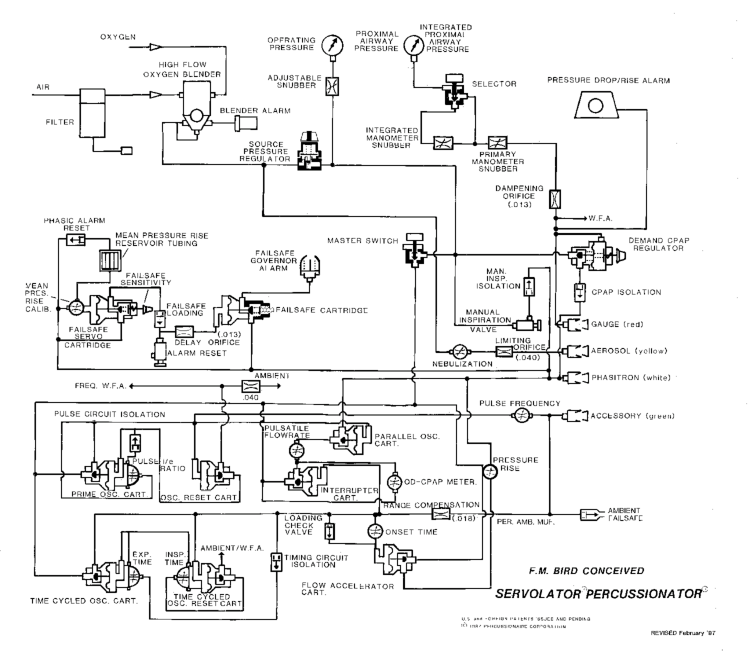
\includegraphics[height=\textheight]{img/circuit-logique.pdf}
	\note {Pas si logique que ça}
\end{frame}

\begin{frame}{Paramètres d'amplitude}
	
\begin{tikzpicture}[
	fleche/.style={
			line width=0.6mm,
			->,
			shorten >=1mm, 
			shorten <=1mm, 
			font=\small,
			vertvdr!60
		},
		cid/.style={
			above=1.35*\ldist,
			align=center,
			font=\tiny
		},
		ampl/.style={
			fill=vertvdr!72
		},
		marker/.style={
			line width=0.3mm,
			vertvdr!60
		},
		index/.style={
			midway,
			below,
			inner
			sep=0,
			font=\tiny,
			scale=0.8
		},
		aug/.style={
			midway,
			above,
			inner
			sep=1mm,
			font=\tiny,
			scale=0.7
		}
]

\colorlet{vertvdr}{green!50!black}

\newcommand{\pexp}{9.5}
\newcommand{\pins}{35.5}
\newcommand{\arrfirst}{1.69}
\newcommand{\arrseccond}{5.68}
\newcommand{\ldist}{7mm}

	\begin{axis} [
			height=0.80\textheight,
			xtick={0,2,4},
			axis x line=bottom,
			axis y line=left,
			enlarge y limits={0.1, upper},
			enlarge x limits={0.05, upper}
		]

		\addplot [
			restrict x to domain=0:6,
			thin,
			]table[x=time, y=Pao] {dat/simvent1.dat};

		\coordinate (A) at (axis cs:1.445,0.1);
		\coordinate (B) at (axis cs:1.445,\pins);

		\draw [marker] (axis cs:0, \pins) -- (axis cs:6, \pins);
		\draw [marker] (axis cs:4, \pexp) -- (axis cs:6, \pexp);

		\draw [fleche] (axis cs:\arrfirst, 0) -- (axis cs:\arrfirst, \pins)
		coordinate [midway] (A);

		\draw [fleche] (axis cs:\arrseccond, \pins) -- (axis cs:\arrseccond, \pexp)
		coordinate [midway] (B);

		\path (A) ++(axis cs: -.7,0) coordinate (C);
		\path (B) ++(axis cs: -.7,-.4) coordinate (D);

	\end{axis}

	\path (C) pic [ampl] {aknob} 
	node [cid] {DEBIT\\PULSE};

	\draw [<->] (C) ++(\ldist, -\ldist) -- ++(0, 2*\ldist) -- ++(-2*\ldist, 0) 
	node [index] {$\blacktriangledown$}
	node [aug] {AUGMENTER}
	;

	\path (D) pic [ampl] {aknob}
	node [cid] {CPAP\\ OSCILLANTE};

	\draw [->] (D) ++(\ldist, \ldist) -- ++(-2*\ldist, 0)
	node [index] {$\blacktriangledown$}
	node [aug] {AUGMENTER}
	;

\end{tikzpicture}

\end{frame}

\begin{frame}[c]{Paramètre de cyclage haute fréquence}
	\centering
	\tikzset{external/remake next}
	\begin{tikzpicture}[
		cid/.style={
			above=1.35*\ldist,
			align=center,
			font=\tiny
		},
		ie/.style={
			fill=black!15
		},
		index/.style={
			midway,
			below,
			inner
			sep=0,
			font=\tiny,
			scale=0.8
		},
		aug/.style={
			midway,
			above,
			inner
			sep=1mm,
			font=\tiny,
			scale=0.7
		},
		plusmoin/.style={
			below,
			inner sep=1mm,
			font=\tiny,
			%scale=0.7,
		},
		false/.style={
			draw=red,
			cross out
		}
]

\newcommand{\ldist}{7mm}

	\path (0,0) pic [ie, pic text=i] {aknob} 
	node [cid] {FREQUENCE\\DE PERCUSSION};

	\draw [->] (0,0) ++(\ldist, \ldist) -- ++(-2*\ldist, 0) 
	node [index] {$\blacktriangledown$}
	node [aug] {AUGMENTER}
	;

	\path (2.5,0) pic [ie, pic text=e] {aknob}
	node [cid] {RAPPORT\\i/e};

	\draw [<->] (2.5,0) ++(\ldist, -\ldist) 
	node [plusmoin] {+}
	-- ++(0, 2*\ldist) 
	-- ++(-2*\ldist, 0) 

	node [index] {$\blacktriangledown$}
	-- ++(0, -2*\ldist) 
	node [plusmoin] {-}
	node [aug] {}
	;

\end{tikzpicture}

\end{frame}

\begin{frame}[c]{Séquence des ajustements}
	\centering
	\centering
\begin{tikzpicture}

	\pic [name=VDR, black!60, scale=0.8] {vdr};

	\begin{scope}[
		every node/.style={
			color=structure!70!black,
			}
			]
	\node (1) at (VDR-e) {1};
	\node (2) at (VDR-i) {2};
	\node (3) at (VDR-F) {3};
	\node (4) at (VDR-O) {4};
	\node (5) at (VDR-I) {5};
	\node (6) at (VDR-E) {6};
	\end{scope}

	\begin{scope}[
		every node/.style={
			yshift=8mm,
			align=center,
			scale=0.5
			}
			]
	\node at (VDR-e) {RAPPORT\\i/e};
	\node at (VDR-i) {FREQUENCE\\DE PERCUSSION};
	\node at (VDR-F) {DEPIT\\PULSE};
	\node at (VDR-O) {CPAP\\OSCILLANTE};
	\node at (VDR-I) {TEMPS\\INSPIRATOIRE};
	\node at (VDR-E) {TEMPS\\EXPIRATOIRE};
	\end{scope}

	\begin{scope}[
		every path/.style={
			structure,
			opacity=0.80,
			line width=0.7mm,
			->
			},
			]
	\draw [] (1) to (2);
	\draw [bend left=27] (2) to (3);
	\draw [bend left=60] (3) to (4);
	\draw [bend left=45] (4) to (5);
	\draw [bend left=45] (5) to (6);
	\end{scope}

\end{tikzpicture}

\end{frame}

\end{document}
